% intro.tex

\section{Introduction}

% background

A barrier is a synchronization primitive used in parallel programming
languages.  The barrier point is a program position at which each thread
of execution enters in parallel and waits to proceed until all threads
have reached the same point.  Figure \ref{fig:barriers} (a) illustrates a barrier
synchronization of the execution of four threads.  Barriers are necessary in
many parallel programs to ensure data integrity between phases of a program
which are to be executed using multiple threads.

\begin{figure*}[hbt]
  \begin{center}
    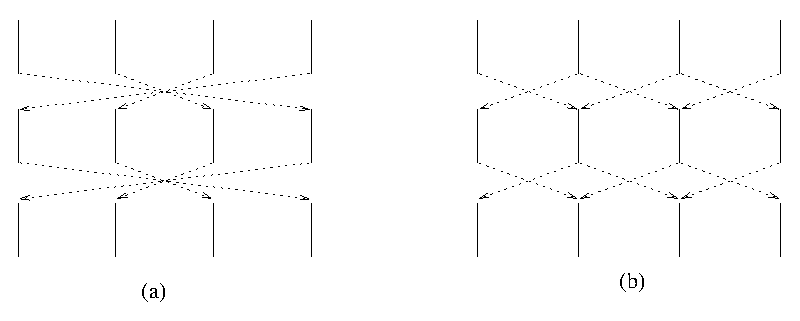
\includegraphics[angle=0, width=0.8\textwidth]{barriers.eps}
    \caption{Barriers}
    \label{fig:barriers}
  \end{center}
\end{figure*}

Barriers are used in both shared and distributed memory programming
models \cite{MPI94} \cite{Sun90} \cite{Kri95}.  We restrict our attention in this paper to software barrier
implementations for cache-coherent shared memory or symmetric
multiprocessor (SMP) systems.  Software barrier implementation for SMP
systems can generally be done using hardware synchronization support such
as fetch-and-add or test-and-set, by using busy-wait polling
techniques or by using some combination of the two.  

In the OpenMP shared memory parallel language specifications\cite{Ope00}\cite{Ope02} , barrier synchronization plays a significant role.  Parallel regions as
well as all of the defined work-sharing constructs are terminated by an
implicit barrier synchronization (which may, in some cases, be avoided using a NOWAIT clause). OpenMP also defines an explicit barrier directive
defined to be used whenever necessary.

In this paper, we will study different ways of implementing
busy-wait barrier synchronization on a multiprocessor system with
shared memory, typically for parallel programming with OpenMP. We use
the EPCC micro-benchmarks\cite{Edi99} to measure performance overhead of the different barrier
implementations discussed here. All of the test data is based on the use of an
explicit barrier, though the results can be applied equally well to implied barriers.

%Our primary hardware system is a 32-way POWER4, which provides good
%performance number for SPECOMP2001\cite{Spe01} while we writing this
%paper. 

In section \ref{overhead}, we describe the POWER4-based system on which
we performed our experiments and the source of some of the costs implicit in
barrier synchronization.  In section \ref{design}, we describe several
implementations of busy-wait synchronization and finally describe our new approach, \emph{distributed counters with local sensor}.  In section \ref{performance}, we show the results of timing and hardware performance monitoring experiments using the various barrier implementations.  Finally, in section \ref{summary}, we summarize our findings and describe future work.

